\section{Architecture}
\label{sec:architecture}
\system{} is an extension of \moodle{} and can be seen as a package of plugins. 
The architecture does not specify how each plugin should be created, but specifies a general structure of the components of the system. 
The complete architecture can be seen in \figref{fig:architecture}.
\begin{figure}[h!t]
	\centering
		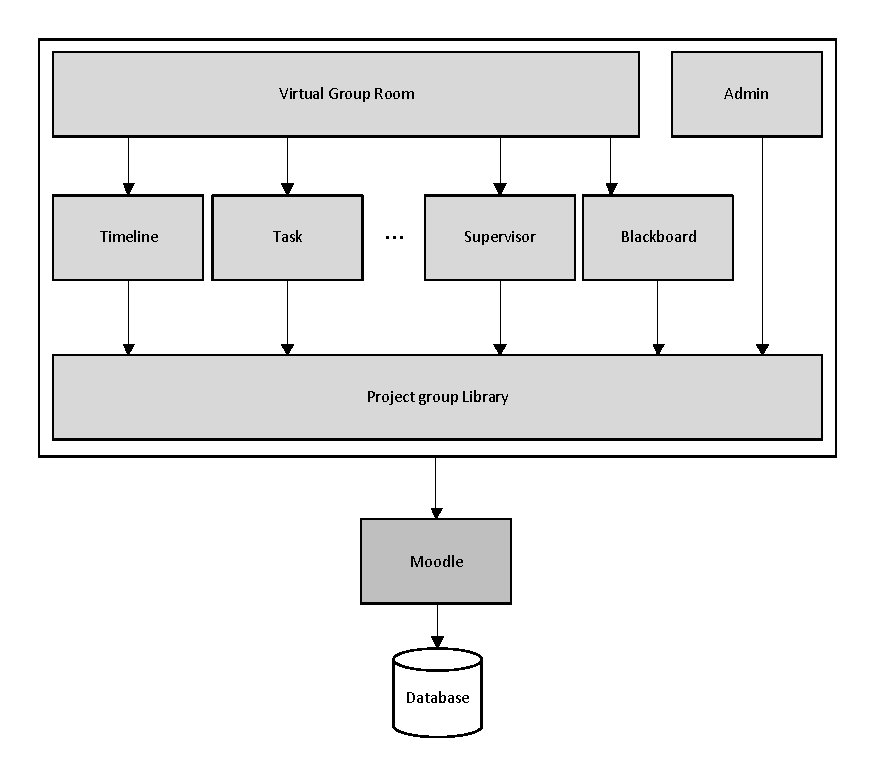
\includegraphics[width=\textwidth]{images/architecture.pdf}
	\morscaption{The overall architecture of MyMoodle}
	\label{fig:architecture}
\end{figure}

The architecture consists of a total of five layers. 
The three uppermost constitute \system{}, they have a common dependency, namely the Moodle platform. 
Layers four and five are Moodle and the Database system respectively.
%Our extension  as a plugin of Moodle and use functions supplied by Moodle to function.

We explain the three uppermost layers as:
\begin{enumerate}
	\item The uppermost layer is the virtual group room and the administration tool.
	%The virtual group room is used for presenting the virtual meeting place for a project group.
	The virtual group room is described in \secref{sec:virtualMeetingPlace}.
	The administrative tool is used by administrative personnel for managing project groups.
	It is described in \secref{sec:groupManagement}.
	This layer is called ``View Layer''.
	\item Directly below the uppermost layer is the middle layer, which consists of the four components: Timeline, Task, Supervisor, and Blackboard.
	These four components are created by our peer-groups and are not explained further.
	We call this layer ``Content Layer'', since the components in this layer generate content for the virtual group room component.
	This layer has three dots in the center in order to show that there exist more components and more can be added here. 
	%An example is the \detdeandrelaver{} that presents the members of the project group. 
	\item Below the Content Layer is the project group library, which contains common functionality.
	This layer handles all communication between the components in the Content Layer.  
	We call this layer the ``Library Layer''.
\end{enumerate}


There are two primary factors we need to consider when planning our architecture. 
Firstly, we are four sub-groups working together. 
This creates the need for a structured way of communicating between the different component and it lets every \subgroup{} know how their component is connected to the rest of the project. 
Secondly, the project should be passed on, which requires an architecture that grants great comprehensibility and extensibility of the project.
%alex -> <@:-D-|-<

It is not possible to make a strict layered architecture due to the Moodle dependency, and the administrative tool, which does not have to use the Content Layer, but depends directly on the project group library and \moodle{}.
We do, however, prohibit ourselves from accessing the database directly, by using the Moodle Database Layer (note that it is not a layer in our architecture) described in \secref{sec:moodleoplatformdbml}.
In \figref{fig:architecture} the dependency from the box encircling \system{} indicates that every component in \system{} depends on the \moodle{} component.
The \moodle{} component consists of the Database Layer as well as the Context System, Capabilities, etc.

%These considerations leads us to design the illustrated architecture in \figref{fig:architecture}.
Note that the relative size of the components do not imply anything, e.g.\ the Moodle component is code wise much larger, than all of the components in \system{} combined, but is illustrated with a rectangle the same size as any of the Content Layer components.













